\begin{frame}[t]
    % \frametitle{Divergence-model choice}
    \frametitle{Inferring co-diversification}

    \vspace{-9mm}

    \begin{minipage}[t][0.1\textheight][c]{1.1\linewidth}
        \begin{adjustwidth}{-0.5em}{}
            \begin{tabular}{ p{2.1cm} p{2.1cm} p{2.1cm} p{2.1cm} p{2.1cm} }
                $m_1$ & $m_2$ & $m_3$ & $m_4$ & $m_5$ \\
            \end{tabular}
        \end{adjustwidth}
    \end{minipage}

    \vspace{-2mm}

    \begin{minipage}[t][0.35\textheight][c]{1.1\linewidth}
        \begin{adjustwidth}{-2.3em}{}
        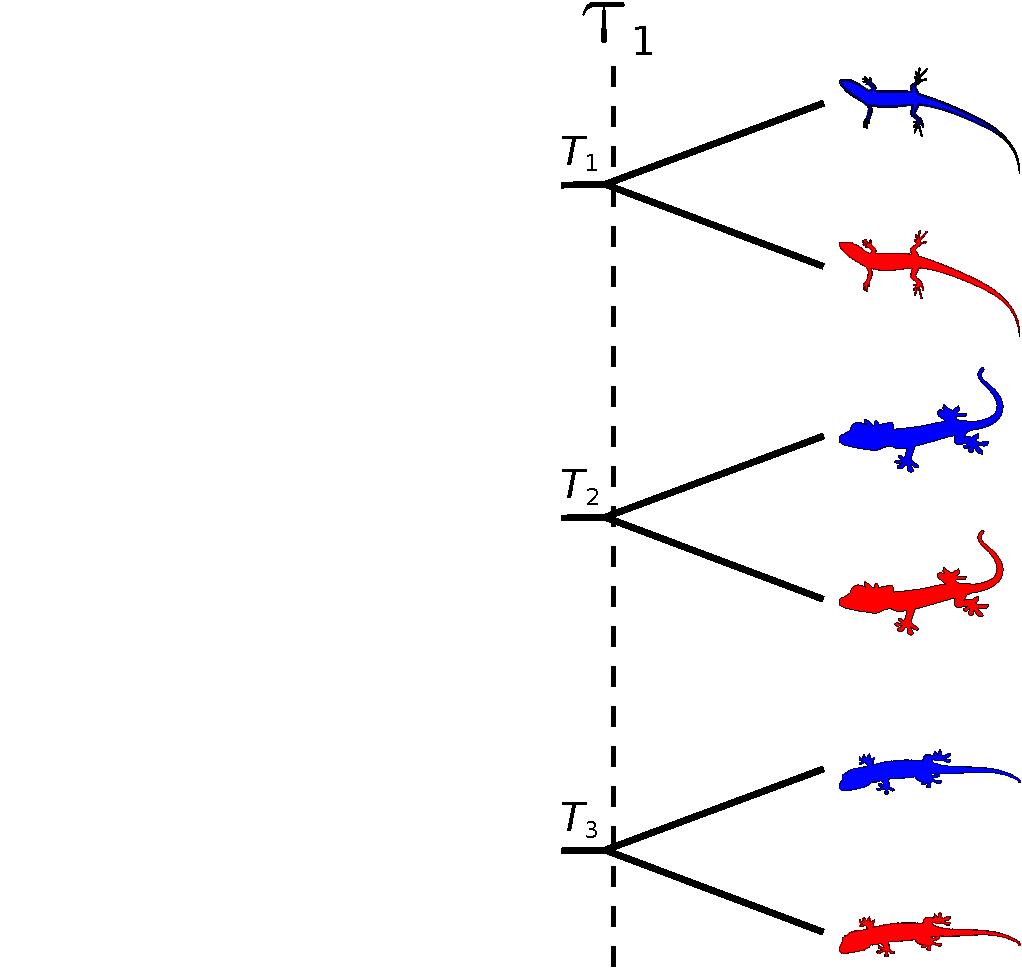
\includegraphics[height=2.0cm]{../images/dmc-cartoon-no-islands-no-sea-levels-shared.pdf}
        \hspace{0.1mm}
        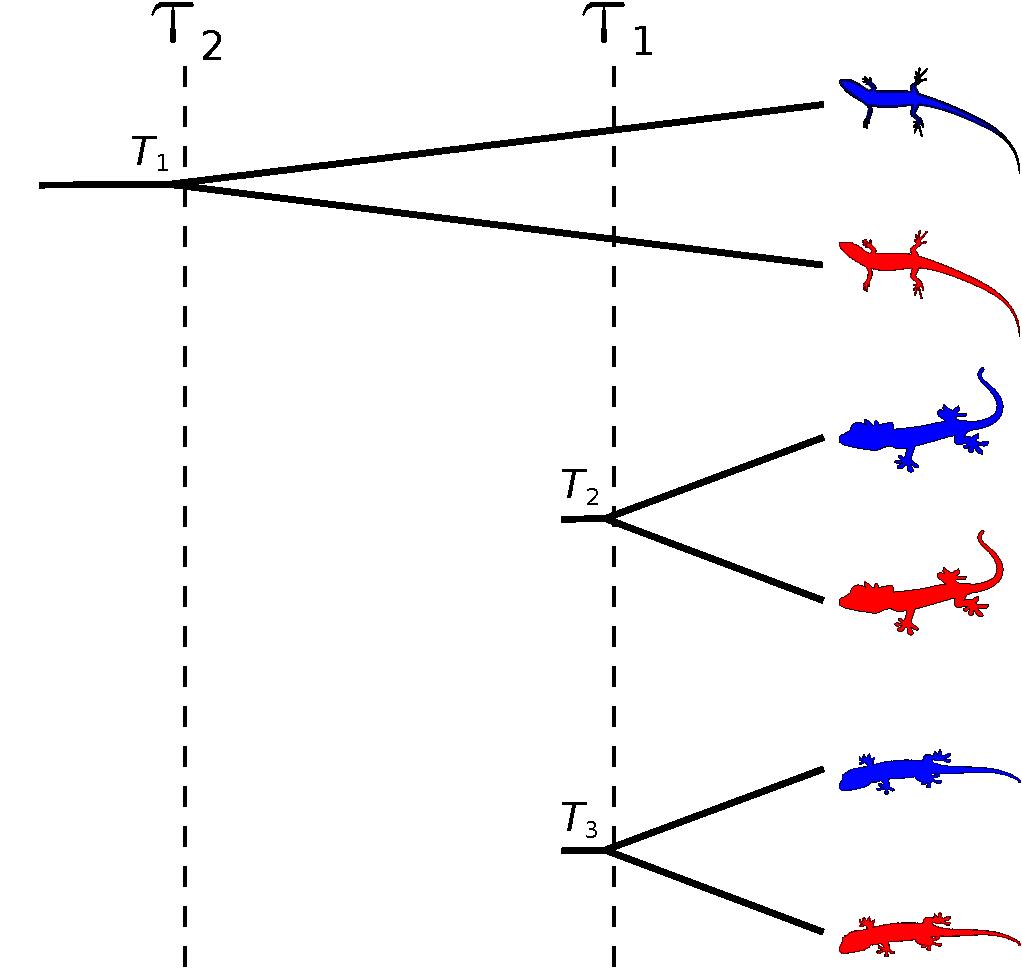
\includegraphics[height=2.0cm]{../images/dmc-cartoon-no-islands-no-sea-levels-2-1.pdf}
        \hspace{0.1mm}
        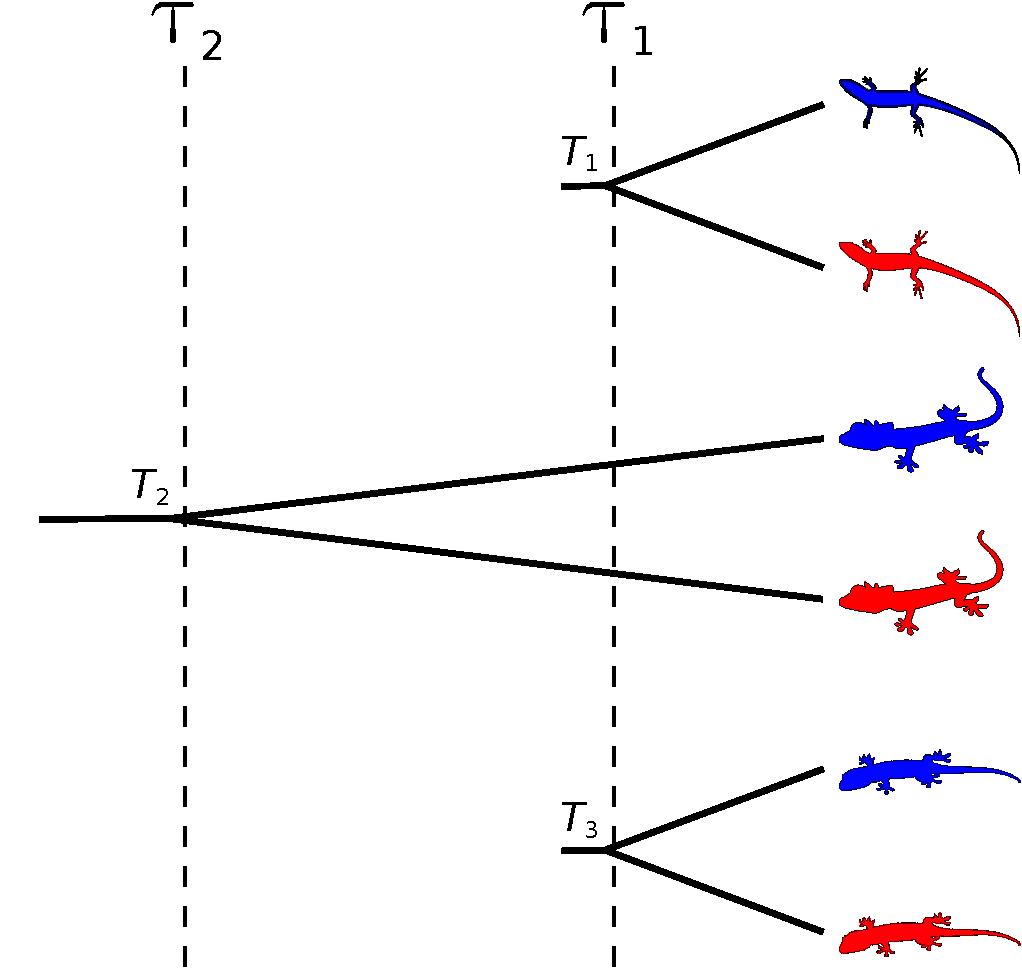
\includegraphics[height=2.0cm]{../images/dmc-cartoon-no-islands-no-sea-levels-2-2.pdf}
        \hspace{0.1mm}
        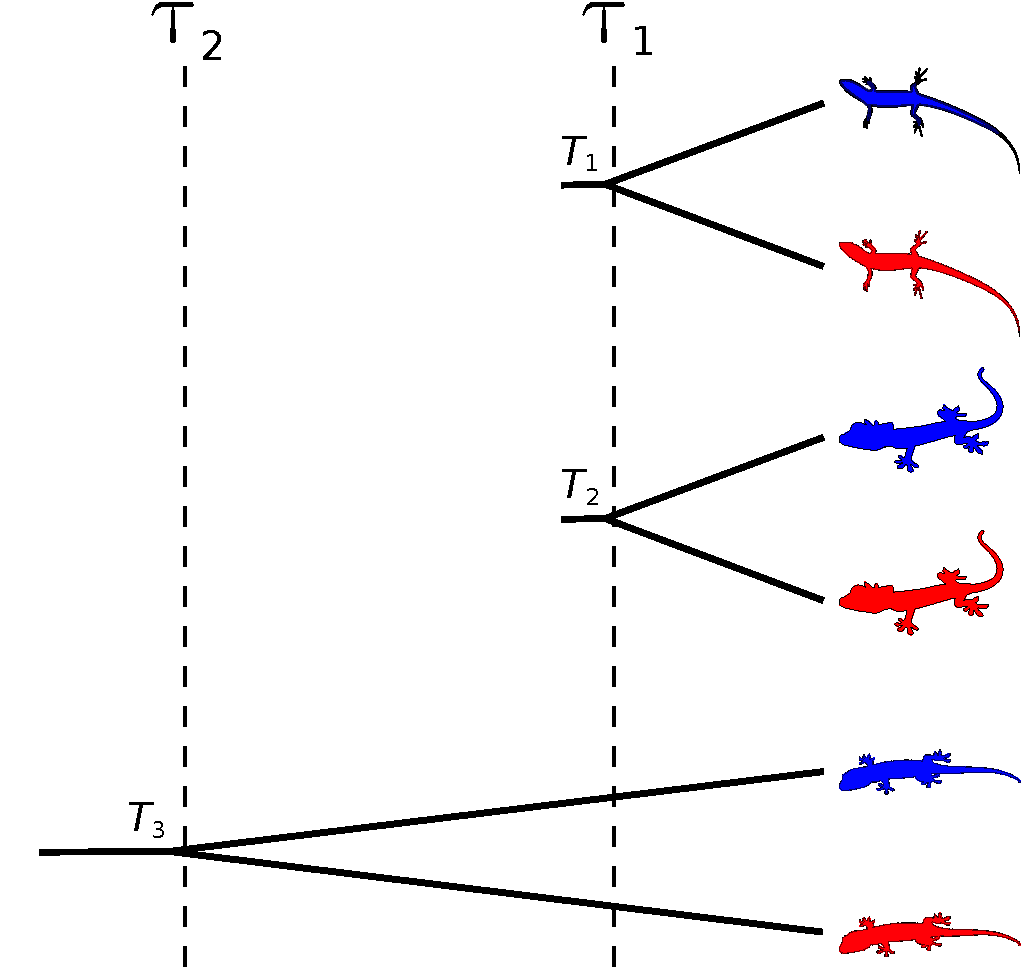
\includegraphics[height=2.0cm]{../images/dmc-cartoon-no-islands-no-sea-levels-2-3.pdf}
        \hspace{0.1mm}
        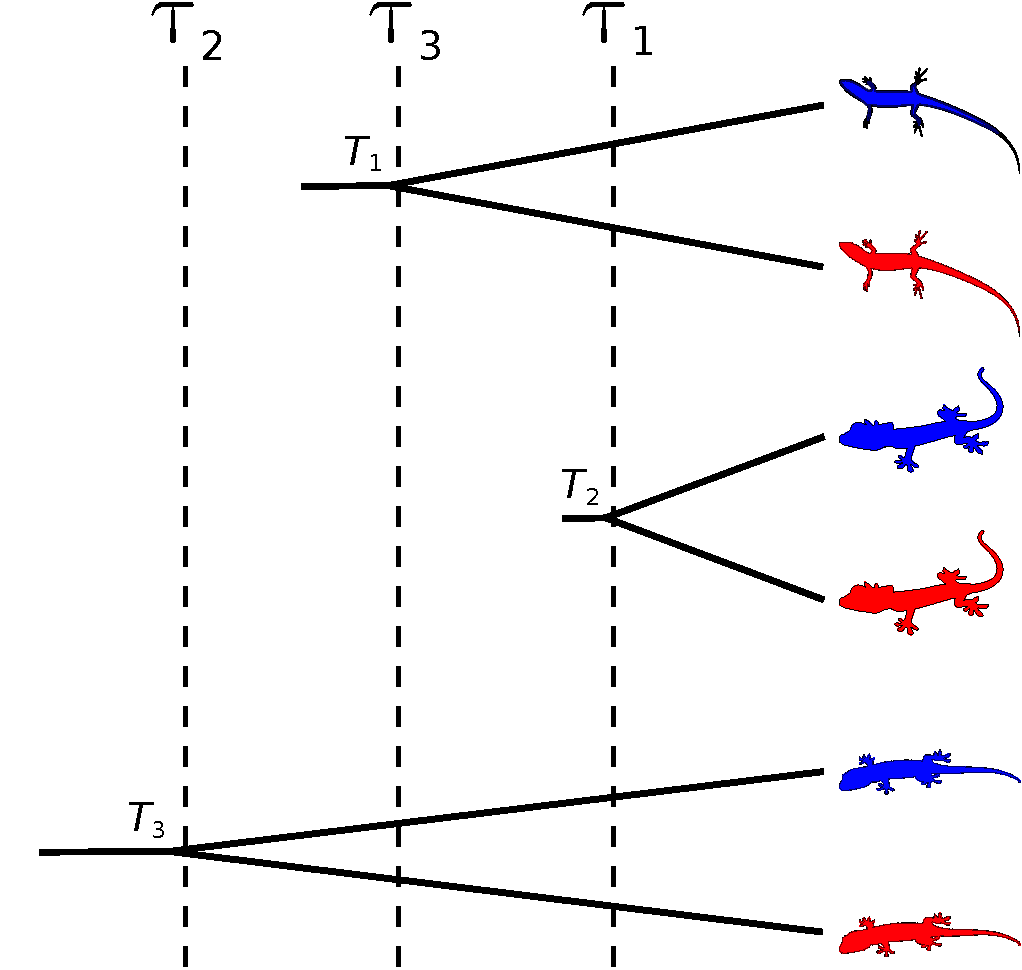
\includegraphics[height=2.0cm]{../images/dmc-cartoon-no-islands-no-sea-levels-general.pdf}
        \end{adjustwidth}
    \end{minipage}

    \vspace{3.5mm}

    \begin{minipage}[t][0.35\textheight][t]{\linewidth}
        \begin{uncoverenv}<2->
            \begin{center}
                We want to infer \textcolor{blue}{\divModel{}} and
                \textcolor{blue}{\divTimeMapVector} given DNA sequence
                alignments
                \textcolor{blue}{\alignmentVector}
            \end{center}
        \end{uncoverenv}

        % \vspace{1mm}

        \begin{uncoverenv}<3->
            \begin{displaybox}[0.85\linewidth]
                % \begin{minipage}[c][0.12\textheight][c]{\linewidth}

                % \[
                %     p(\divTimeMapVector,
                %       \divModel{i},
                %       \allParameters{}
                %       \given \alignmentVector)
                %       =
                %     \frac{
                %         p(\alignmentVector \given
                %           \divTimeMapVector,
                %           \allParameters{},
                %           \divModel{i})
                %         p(\divTimeMapVector,
                %           \allParameters{}
                %           \given \divModel{i})
                %         p(\divModel{i})
                %         }{p(\alignmentVector)}
                % \]
                % \vspace{-1mm}
                % \end{minipage}
                \begin{minipage}[c][0.1\textheight][c]{\linewidth}
                    \begin{onlyenv}<3>

                        \vspace{3.5mm}

                        \[
                            p(
                              \divTimeMapVector,
                              \allParameters{}
                              \given \alignmentVector, \divModel{i})
                              =
                            \frac{
                                p(\alignmentVector \given
                                  \divTimeMapVector,
                                  \allParameters{},
                                  \divModel{i}
                                  )
                                  p(
                                    \divTimeMapVector,
                                    \allParameters{}
                                    \given \divModel{i}
                                    )
                                }{p(\alignmentVector \given \divModel{i})}
                        \]
                    \end{onlyenv}
                    \begin{onlyenv}<4>

                        \vspace{3.5mm}

                        \[
                            p(\divModel{i} \given \alignmentVector) =
                            \frac{
                                p(\alignmentVector \given \divModel{i})
                                p(\divModel{i})
                            }{
                                \sum_{i} p(\alignmentVector \given \divModel{i})
                                p(\divModel{i})
                            }
                        \]
                    \end{onlyenv}
                    \begin{onlyenv}<5->

                        \vspace{2mm}

                        \[
                            p(\alignmentVector \given \divModel{i}) =
                            \int_{\divTimeMapVector} \int_{\allParameters{}}
                            p(\alignmentVector \given \divTimeMapVector, \allParameters{}, \divModel{i})
                            p(\divTimeMapVector, \allParameters{} \given \divModel{i})
                            d\divTimeMapVector d\allParameters{}
                        \]
                    \end{onlyenv}
                    % \begin{onlyenv}<16>
                    %     \vspace{-2mm}
                    %     \begin{center}
                    %     \msb: Approximate Bayesian computation (ABC)
                    %     \end{center}
                    % \end{onlyenv}
                \end{minipage}
            \end{displaybox}
        \end{uncoverenv}

        \vspace{-1mm}

        \begin{uncoverenv}<6->
            \begin{center}
                \begin{itemize}
                    \small
                    \item Dirichlet-process prior (DPP) over all possible divergence
                        models
                    % \item<2-> Flexible priors on continuous parameters to avoid strongly
                    %     weighted posteriors
                    \item Multi-processing interface to accommodate genomic datasets
                \end{itemize}
            \end{center}
        \end{uncoverenv}
    \end{minipage}
\end{frame}

